%
% $RCSfile: overview.tex,v $
%
% Copyright (C) 2002-2008. Christian Heller.
%
% Permission is granted to copy, distribute and/or modify this document
% under the terms of the GNU Free Documentation License, Version 1.1 or
% any later version published by the Free Software Foundation; with no
% Invariant Sections, with no Front-Cover Texts and with no Back-Cover
% Texts. A copy of the license is included in the section entitled
% "GNU Free Documentation License".
%
% http://www.cybop.net
% - Cybernetics Oriented Programming -
%
% http://www.resmedicinae.org
% - Information in Medicine -
%
% Version: $Revision: 1.1 $ $Date: 2008-08-19 20:41:08 $ $Author: christian $
% Authors: Christian Heller <christian.heller@tuxtax.de>
%

\subsection{Overview}
\label{overview_heading}
\index{Medical Informatics Working Groups}
\index{Deutsches Institut fuer Normung}
\index{DIN}
\index{Comite Europeen de Normalisation}
\index{CEN}
\index{International Organization for Standardization}
\index{ISO}

Figure \ref{groups_figure} shows the medical informatics working groups of
important standardisation organisations, namely the:

\begin{itemize}
    \item[-] \emph{Deutsches Institut fuer Normung} (DIN)
    \item[-] \emph{Comite Europeen de Normalisation} (CEN)
    \item[-] \emph{International Organization for Standardization} (ISO)
\end{itemize}

\begin{figure}[ht]
    \begin{center}
        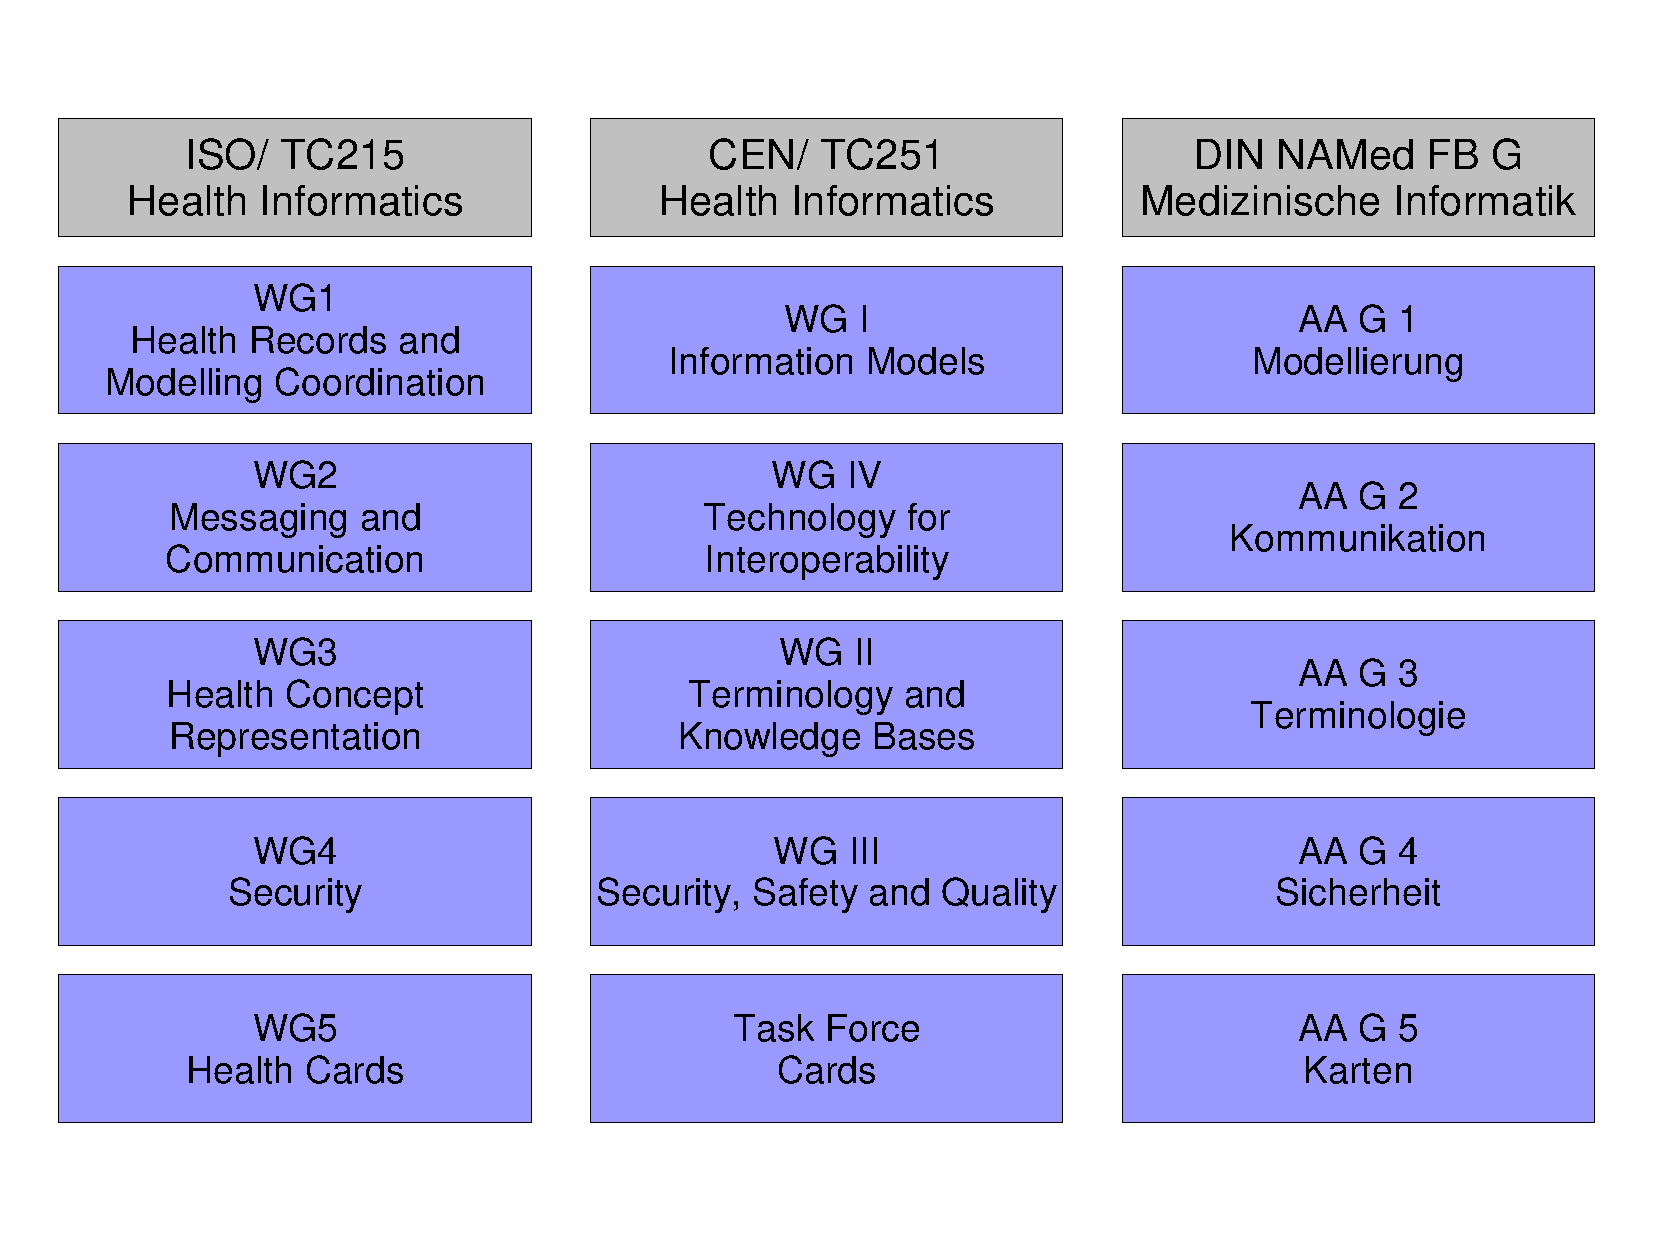
\includegraphics[scale=0.3,angle=-90]{graphic/groups.pdf}
        \caption{Medical Informatics Working Groups of DIN/ CEN/ ISO \cite{atgexpertsreport}}
        \label{groups_figure}
    \end{center}
\end{figure}

The structure of the following sections is chosen after this systematics.
Standards for \emph{Health Record Modelling} will be described first, followed
by those for \emph{Messaging and Communication} and a section on
\emph{Terminology- and Coding Systems}. \emph{Imaging-}, \emph{Health Card-}
and further standards are mentioned afterwards. General remarks on current
\emph{Standards Development Processes} follow. Reflections on the
\emph{Implications} of standards on the development of \emph{Res Medicinae}
will conclude the topic.
